\chapter{Анализ задачи}

\section{Обзор существующих реализаций палитр команд}\label{analogs}

Впервые палитра команд появилась 1 июля 2011 году в редакторе Sublime Text
2~\cite{sublimetext2changelog}. Вслед за этим подобный функционал был реализован
в некоторых других программах. Таких, как:
\begin{itemize}
	\item Atom\cite{atom},
	\item VSCode\cite{vscode},
	\item JupyterLab\cite{jupyterlab}.
\end{itemize}

Но это были лишь единичные случаи. В апреле 2017 года появилась альфа-версия
приложения Plotinus\cite{plotinus}, которое позволяет добавлять палитру команд в
любое приложение, использующее графическую библиотеку GTK.

Таким образом можно наблюдать, что частные решения начинают заменяться более
универсальными. Однако на текущий момент эти решения не позволяют покрыть
большинство областей т.к. ограничены лишь программами с GTK, который
используется не более чем в половине прикладных приложений для ОС Linux и
занимает совсем малую долю среди приложений для ОС Windows.

\begin{figure}[h]
	\centering
	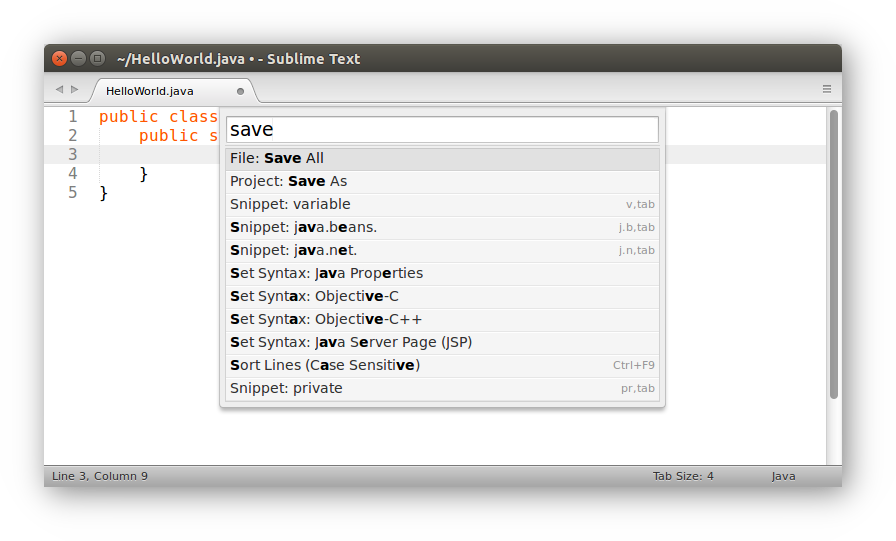
\includegraphics[width=\textwidth]{SublimeText}
	\label{sublimetext}
	\caption{Sublime Text}
\end{figure}

\begin{figure}[h]
	\centering
	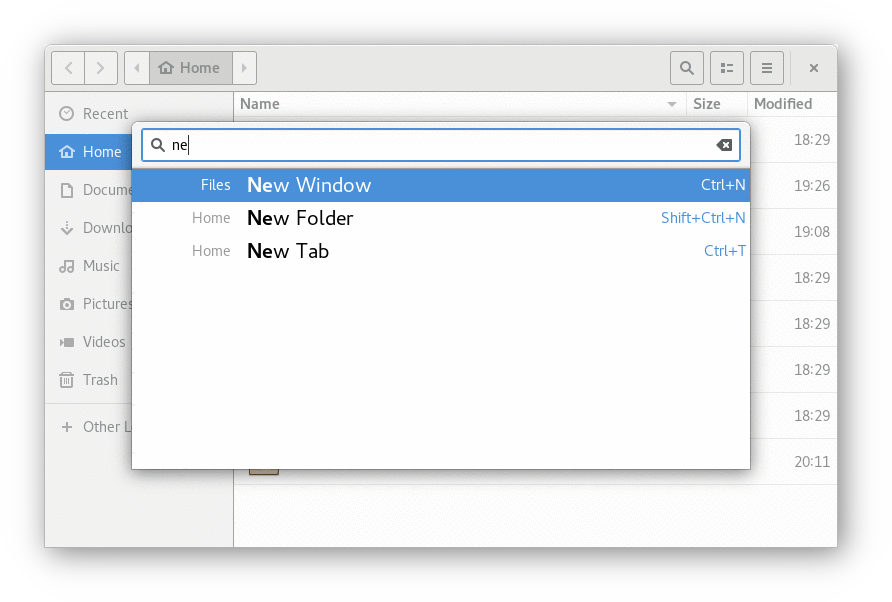
\includegraphics[width=\textwidth]{Plotinus}
	\caption{Plotinus}
\end{figure}

\section{Qt}

Qt — это кроссплатформенный фреймворк для разработки программного обеспечения
на языке программирования C++\cite{qtabout}. Он содержит множество библиотек для
упрощения реализации прикладных задач. Благодаря кроссплатформенности данный
фреймворк позволяет запускать написанное с его помощью ПО на многих операционных
системах путем обычной сборки проекта без внесения изменений в исходный код
самой программы. Отличительной особенностью Qt является наличие метаобъектного
компилятора, который запускается до основной компиляции и генерирует
вспомогательный код. Такой подход позволил добавить частичную поддержку такого
инструмента как рефлексия.

Qt включает в себя следующие модули:

\begin{itemize}
    \item Qt Core — базовые классы, обеспечивающие рефлексию, работу со
        строками, механизмы владения и т.п. Используются всеми остальными
        модулями;
    \item Qt Network — классы, позволяющие легко писать переносимый код для
        работы с сетью;
    \item Qt SQL — классы, предоставляющие удобный программный интерфейс для
        работы с различными реляционными БД;
    \item Qt Multimedia — классы, для работы с данными (аудио и видео),
        устройствами (камеры, микрофоны);
    \item Qt GUI — классы, позволяющие реализовать приложения с графическим
        интерфейсом.
\end{itemize}

В ОС Linux библиотеки GTK и Qt являются двумя наиболее популярными средствами
для реализации приложений с графическим интерфейсом. Т.к. средство для
добавления палитры команд уже есть для GTK, в данной работе будет рассмотрена
такая возможность для Qt.

События в Qt — это объекты, унаследованные от абстрактного класса \code{QEvent},
которые представляют действия, произошедшие внутри приложения, либо созданные в
результате активности пользователя, о которых приложение должно знать. События
могут быть получены и обработаны любым экземпляром подкласса \code{QObject}, но
они особенно актуальны для графических элементов.

Обычно события доставляются объектам через вызов виртуальных функций. Если
разработчик хочет заменить функцию базового класса, он должен реализовать
всю обработку самостоятельно. Однако, если нужно только расширить
функциональность то разработчик реализует нужное расширение, а затем вызывает
базовый класс, чтобы обеспечить поведение по умолчанию для тех случаев, которые
он не хочет обрабатывать.

Не всегда в классе имеется нужная функция для события. Наиболее распространенный
пример — обработка нажатия клавиш, для которой нет соответствующей виртуальной
функции. Для обработки таких событий нужно переопределить метод
\code{QObject::event()}. Он является общим обработчиком событий, и позволяет
выполнить дополнительные действия до или после обработки по-умолчанию.

\section{Организация работы приложения}

Система управления должна позволять контролировать множество приложений. Для ее
реализации лучше всего подходит клиент-серверная архитектура. Для каждого
целевого приложения будет запускаться отдельный клиент, который будет заниматься
сбором информации об элементах управления и передавать ее на сервер.

В качестве сервера будет выступать приложение, которое запускает целевые
приложения вместе с клиентами. После этого сервер принимает входящее соединение
от клиента и отображающее окно поиска элемента для текущего активного окна.

Для удобной работы окно поиска должно отображаться окно поверх работающего
приложения. И в нем должен производится нечеткий поиск.

\subsection{Добавление логики в стороннее приложение}

Разработчики любого приложения не могут учесть желания и капризы всех
пользователей. Благодаря этому приложения не превращаются в комбайны, которые
невозможно было бы поддерживать. Разработчики могут убрать какую-то деталь,
которая нужна малому проценту людей. Ведь надо тратить время на исправление
ошибок в ней. А иногда эти специфичные функции могут даже замедлять работу всего
приложения. В таком случае пользователи могут захотеть добавить какую-то
дополнительную логику или функцию в основное приложение.

Подходы делятся на два типа:
\begin{itemize}
	\item добавление функции на этапе сборки приложения;
	\item добавление функции в момент выполнения программы.
\end{itemize}

Целью данной работы является добавление функциональности в максимальную группу
приложений. Первый же подход исключает такую возможность для приложений с
закрытым исходным кодом. К тому же при первым подходом может пользоваться только
квалифицированный пользователь. И то, ему пришлось бы пересобирать каждое
приложение в которое он хотел бы добавить нужную функциональность.

Программный модуль подключаемый к уже существующему приложению называется
плагином. Для добавления возможности подключения плагинов разработчики программы
должны или написать свою систему плагинов или воспользоваться готовой. Так,
например, библиотека GTK, начиная с третьей версии, предоставляет возможность
запускать приложения с дополнительными модулями, которые могут расширять
функциональность приложения. Этим воспользовались разработчики библиотеки
Plotinus, реализовав возможность добавления палитры команд в любое приложение,
использующее GTK.

Qt предоставляет возможность встраивать дополнительную
функциональность в приложение, но для этого оно должно иметь специальный код по
загрузке дополнительных модулей, который в большинстве случаев не используется
(для подтверждения можно сравнить число github репозиториев использующих
Qt\cite{githubqt} и использующих функцию Qt для работы с
плагинами\cite{githubqpluginloader}. Соотношение примерно 1:100).

Кроме штатных средств добавления функционала на уровне приложения есть и более
низкоуровневые. Так например в Windows есть функция автоматизации
интерфейса UI Automation\cite{windowsuiautomation}, которая изначально была
добавлена для увеличения доступности приложений людям с ограниченными
возможностями. Этот же функционал не такой богатый, как функционал плагинов
(тут есть возможность работы только с видимыми элементами интерфейса), но зато
доступен для любого приложения, использующего стандартные элементы управления.
В случае использования Linux, к сожалению, нет такой возможности на уровне ОС
или графической оболочки.

\subsection{Внедрение модуля}

Рассмотрим в общих чертах механизм работы графического приложения. На
рис.~\ref{fig:gui} изображено как происходит взаимодействие между элементами
графического приложения и пользователем.

\begin{figure}
	\centering
	\begin{tikzpicture}[
        ->,>=stealth',node
        distance=1.5cm, semithick,
        every edge/.append style={<->}
    ]

    \tikzstyle{block} = [rectangle,draw,minimum height=0.8cm]

    \node[block] (user) {Пользователь};
    \node[block] (x11) [below of=user] {Графическая подсистема X11};
    \node[block] (lib) [below of=x11] {Графическая библиотека Qt};
    \node[block] (app) [below of=lib] {Приложение};
    \path[]
        (user) edge (x11)
        (x11) edge (lib)
        (lib)  edge (app)
    ;

\end{tikzpicture}
\\
	\caption{Взаимодействие элементов ГИП и пользователя}\label{fig:gui}
\end{figure}

Исходя из данной упрощенной схемы можно предложить еще одно способ добавить
функциональность — создание события от графической библиотеки, которое будет
передано приложению.

\subsection{Механизм подмены функций}

При запуске приложения загрузчик получает из приложения список всех используемых
динамических библиотек, загружает их в память. Затем получает адреса всех
экспортированных функций динамической библиотеки и сохраняет их для последующего
вызова.

Загрузчик ld, который используется в Linux и FreeBSD позволяет загружать
дополнительные динамические библиотеки, кроме тех, кто запрашивает приложение.
Эта дополнительная библиотека загружается раньше всех остальных, что позволяет
ей подменять функции из других библиотек. Это происходит потому, что при поиске
адреса определенной функции берется первый подходящий.

\subsection{Способ получения информации об элементах}

Для получения информации об элементах интерфейса можно загрузить специальную
библиотеку, которая будет регистрировать создания, изменения и удаления
элементов интерфейса. Затем собранная информация будет передавать на сервер для
последующей работы.

Также данная библиотека может создавать ложные события по командам, приходящим с
сервера. Таким образом можно имитировать нажатия кнопок, открытие меню и т.п.

Пользовательский интерфейс через специальное API сможет получать от сервера
информацию о доступных элементах в текущем приложении. После того, как
пользователь произвел выбор, вызывается специальная функция на стороне сервера,
которая приводит к отправке команды клиенту.

\subsection{Реализация кода для подмены функции}

Для внедрения библиотеки требуется реализовать заглушки для функций Qt, которые
будут вызывать специальный обработчик, а затем продолжать нормальное выполнение
функции. Дополнительную сложность создает то, что библиотека Qt написана на
языке C++, который из-за поддержки классов и перегрузок функций использует т.н.
«искажение имен» (name mangling). Таким образом чтобы создать такой обработчик
нужно специальным образом сконструировать имя функции исходя из имени класса,
метода, набора параметров и возвращаемого значения.

Создание таких обработчиков является рутинной работой в которой человек легко
может допустить ошибку. Поэтому вместо ручного написания каждого обработчика
нужно написать генератор, который может добавить нужные обработчики имея
минимальный и необходимый набор данных (имя класса, метода и т.д.).

\section{Постановка задачи}

Требуется разработать набор программ, которые в комплексе будут решать следующие
задачи:

\begin{itemize}
	\item запускать целевые приложения в специальном окружении;
	\item собирать информацию о существующих элементах графического приложения;
	\item сохранять информацию о всех запущенных приложениях;
	\item отображать пользователю окно для поиска и выбора элемента;
	\item активировать выбранный пользователем элемент.
\end{itemize}

Исходя из приведенного выше анализа следует, что задачи должны быть сгруппированы
в набор программ. Он должен быть реализован в виде следующих элементов:

\begin{enumerate}
	\item\label{lib} Библиотека для внедрения и сбора информации в конкретном
		приложении.
	\item Приложение для сохранения информации, полученной из нескольких
		приложения с библиотекой из п.\ref{lib}.
	\item Графический интерфейс для запуска приложений и отображения окна
		палитры команд.
\end{enumerate}

\section{Архитектура приложения}

Подходящая архитектура для такой задачи была предложена мной в одной из прошлых
работ\cite{polshakovinject}. На рис.~\ref{fig:arch} изображена схема
взаимодействия данного комплекса программ. На схеме изображены следующие
действия:
\begin{enumerate}
    \item Перехват функции создания элемента интерфейса
    \item Оповещение о создании элемента
    \item Вызов оригинальной функции графической библиотеки
    \item Отображение элемента управления
    \item Передача информации об элементе приложению управления
    \item Отображение палитры команд
    \item Выбор команды
    \item Вызов функции для выполнения команды
    \item Передача команды к выполнению
    \item Вызов функции активации окна целевого приложения
    \item Активация окна
    \item Перехват функции обработки события
    \item Вызов функции обработки события
    \item Вызов функции для выполнения команды
    \item Выполнение команды
\end{enumerate}

\begin{figure}
	\centering
	\begin{tikzpicture}[
        ->,>=stealth',node
        distance=2cm, semithick
    ]

    \tikzstyle{block} = [rectangle,draw,minimum height=0.8cm]

    \node[block] (preload) {Подгружаемый модуль};
    \node[block] (lib)    [above of=preload] {libQtWidgets};
    \node[block] (x11)    [above of=lib]     {X11};
    \node[block] (server) [left=2cm of preload] {Сервер управления};
    \node[block] (app)    [below of=preload] {Целевое приложение};

    \node[block] (ctrl) [above of=server] {Приложение управления};
    \node[block] (user) [above of=ctrl] {Пользователь};

    \path[]
        (app)     edge[bend left]     node[left]  {1} (preload)
        (preload) edge[bend left=5]   node[below] {2} (server)
        (preload) edge[bend left]     node[left]  {3} (lib)
        (lib)     edge[bend left]     node[left]  {4} (x11)
        (server)  edge[bend left]     node[left]  {5} (ctrl)
        (ctrl)    edge[bend left]     node[left]  {6} (user)
        (user)    edge[bend left]     node[right] {7} (ctrl)
        (ctrl)    edge[bend left]     node[right] {8} (server)
        (server)  edge[bend left=5]   node[above] {9} (preload)

        (server.north east)  edge    node[above]{10} (x11)

        (x11)     edge[bend left]     node[right] {11} (lib)
        (lib)     edge[bend left]     node[right] {12} (preload)
        (preload) edge[bend left]     node[right] {13} (app)
        (preload) edge[bend right=75] node[right] {14} (lib)
        (lib)     edge[bend left=80]  node[right]  {15} (app)
    ;

\end{tikzpicture}
 \\
	\caption{Общий обзор архитектуры}\label{fig:arch}
\end{figure}
